\documentclass{jarticle}
\usepackage[dvipdfmx]{graphicx}
\usepackage{here}
\usepackage{listings,jlisting}
\usepackage{amsmath}

\lstset{
  basicstyle={\ttfamily},
  identifierstyle={\small},
  commentstyle={\smallitshape},
  keywordstyle={\small\bfseries},
  ndkeywordstyle={\small},
  stringstyle={\small\ttfamily},
  frame={tb},
  breaklines=true,
  columns=[l]{fullflexible},
  numbers=left,
  xrightmargin=0zw,
  xleftmargin=3zw,
  numberstyle={\scriptsize},
  stepnumber=1,
  numbersep=1zw,
  lineskip=-0.5ex
}

\title{{システム実験}\\実験後期第2回レポート}
\author{6119019056 山口力也}
\date{2019/10/17日提出}
\begin{document}
\maketitle
\section{課題11.2.1}
演習11.2.2でのシリアル通信のプログラム(プログラム2)では,プログラム中で50msのdelayを行っていた.このdelayを行わない場合,シリアル通信の結果がどのように変化するか確認せよ. \\
表示内容がどのように変わったか,画面のスクリーンショットを示して解説せよ.また,結果が変わった原因を考察せよ. \\
以下図\ref{fig:kadai11-2-1}に画面のスクリーンショットを示す.

\begin{figure}[H]
\begin{center}
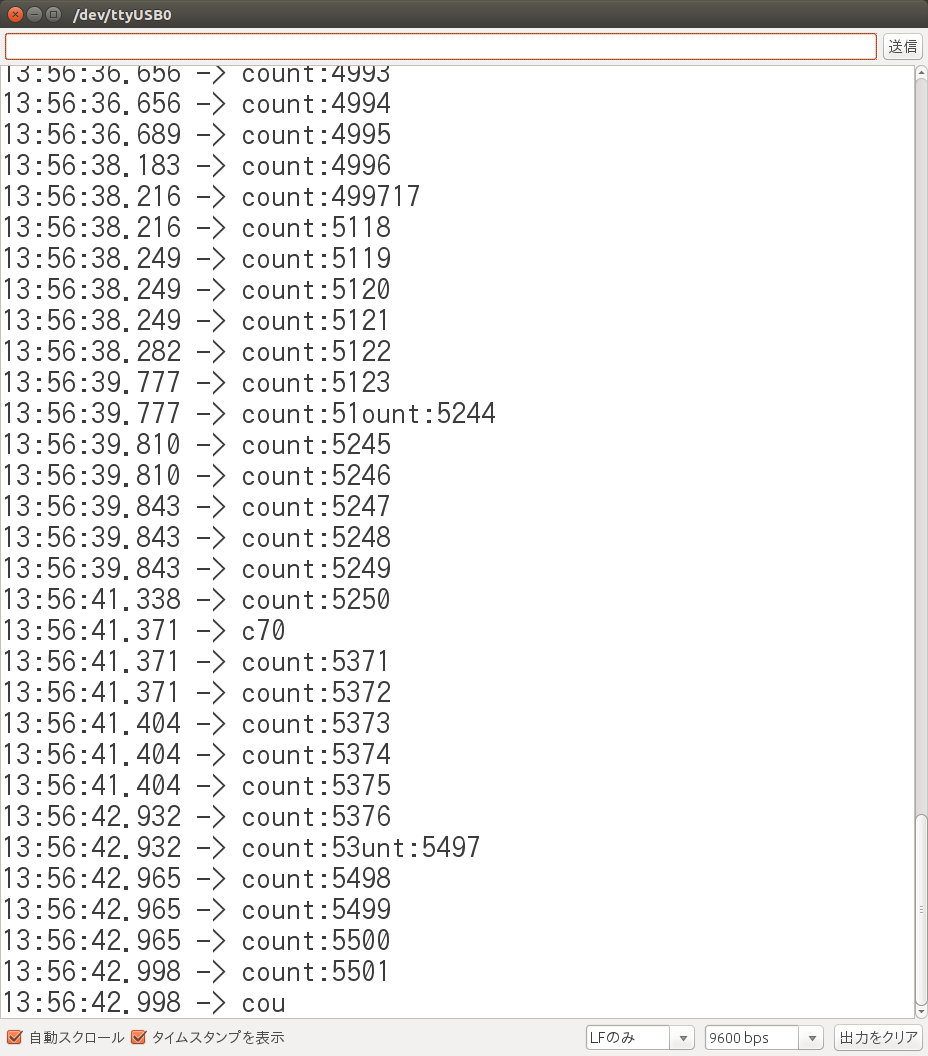
\includegraphics[width=7.0cm]{images/kadai11-2-1.png}
\caption{課題11.2.1の結果}
\label{fig:kadai11-2-1}
\end{center}
\end{figure}

delayを行わない場合,システムモニタの表示に不具合が起きた.これは,Arduino側でシリアル通信により文字列を送信してからシリアルモニタに表示されるまでの間に次の文字列が送信されることが原因だと考えられる.

\section{課題11.2.2}

